\documentclass[11pt,a4j,ascmac]{jarticle}
\usepackage{epsf}
\usepackage[dvips]{graphicx}

\setlength{\textheight}{25cm}
\setlength{\textwidth}{16cm}
\setlength{\topmargin}{-2.5cm}
\setlength{\oddsidemargin}{0mm}
\setlength{\parindent}{0pt}
\setlength{\parskip}{3mm}

\title{7月 進捗確認会報告資料\\
Augumented Autencoderを用いた姿勢推定の調査}


\西暦     
\author{安井 理}
\date{\today}
\begin{document}
\maketitle

\section{はじめに}

\ 前回の進捗報告会までに調べてきた,ARマーカの座標推定のためのSSD-6D論文が,実装を行うことが難しいという事が分かったため,別の方法を考えることにした. \\
\ 今回調べてきた論文も前回同様6次元の姿勢推定を行うための手法であるが,方法としては前回調べてきた論文とは違い検出と推定を分けて考えられた手法である. 調べてきた論文では,実際にコードがすべてGit-hubに記載されており,実装することが可能なので,この論文を軸に引き継ぎをした鈴木さんの研究と合わせて自分の研究の目標を明確にし進めることにした. 最終的な研究目標としては鈴木さんの研究(Faster-RCNN)を用いた検出と組み合わせて座標推定を実現できるようにしていこうと考えている.



\section{進捗報告}




\subsection{調査内容}

\begin{description}
  \item  ・implicit 3d orientation learning for 6d object detection from rgb images の論文調査
 \item ・Augumented Autencoderの手法理解
 \item ・検出推定の手法理解
 \item ・実装に向けた環境作り
\end{description}


今回調査した手法及び論文は以下である.
 
\begin{description}
    \item ・implicit 3d orientation learning for 6d object detection from rgb images 
    \item ・Domain Randomization 
\end{description}


\subsection{今回扱う6次元推定の概要}
\  implicit 3d orientation learning for 6d object detection from rgb images の論文は,ECCV2018のBest paperに選ばれた6次元物体検出の論文.\\
\ 6D物体検出は,3次元空間座標だけでなく3方向の向き姿勢情報も含んだ検出問題であり,高速に推定を行えることに加えて,6Dのラベル付き教師データがなくても学習可能な手法である.6Dラベル付き教師データの代わりに、検出対象となる物体の3D CADデータが必要となる. 全体の処理の流れ図1としては,まず入力となるRGB画像に対してSSDを用いて対象物体のBounding Boxを推定,その後,推定されたBounding Box領域から物体の姿勢情報を推定するという処理を行う,後半のBounding Box領域から物体の姿勢情報を推定する部分が今回自分の研究に取り入れようと考えている方法で,Augmented AutoEncoder(以降AAE)という手法が用いられている.\\   
      \begin{figure}[htpp]
      \centering
      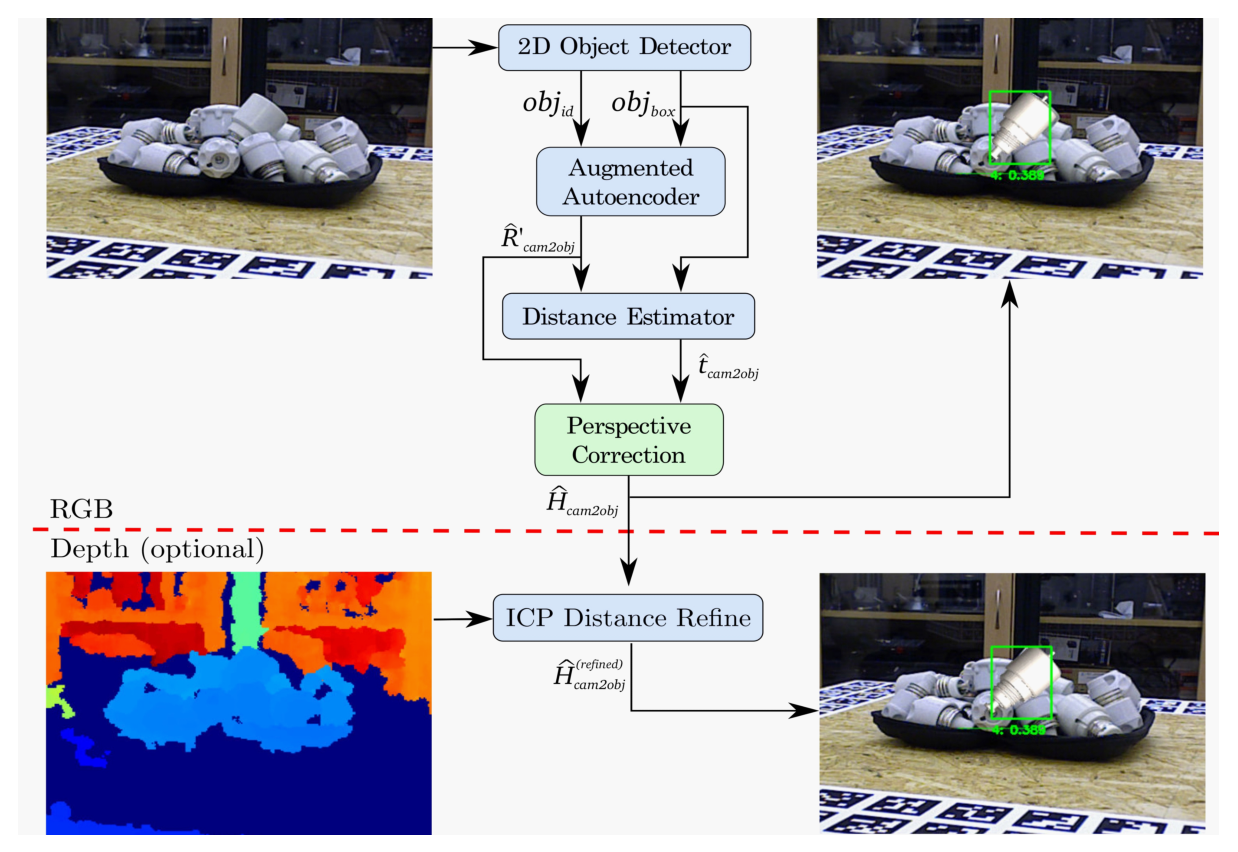
\includegraphics[width=80mm]{pic1.eps}
      \vspace*{20mm}
      \caption{全体の流れ.}
      \label{fig:2d_pose_estimation}
      \end{figure}

\subsection{トレーニング}

\  あらかじめAugumented Autencoder(AAE)を使い検出したい物体の3Dモデルを作成し様々な視点でトレーニングするトレーニングの流れを図2に示す.まず等間隔に3Dモデル物体を回転させ,すべての角度の視点(2562点)と物体の各回転座標のコード.一つの視点につき36点を用意 ,AAEにかけ潜在変数z ∈R128を生成して( zi , Ri)を一つの物体IDに92232個記録していく.\\ \\ \\

      \begin{figure}[htpp]
      \centering
      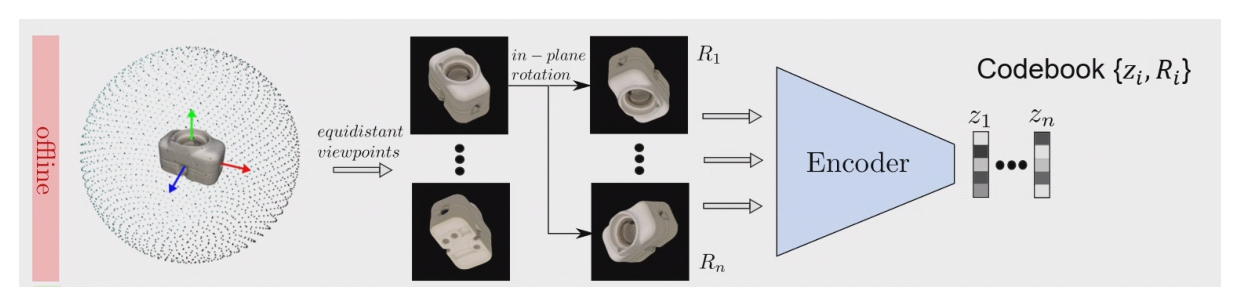
\includegraphics[width=80mm]{pic2.eps}
      \vspace*{40mm}
      \caption{トレーニングの全体像.}
      \label{fig:2d_pose_estimation}
      \end{figure}





\subsubsection{Domain Randomization}
\ 今回扱うAAEにはDomain Randomizationという考え方が取り入れられている.この手法の目的は,テスト時にモデルが実世界のデータに一般化できるよう,環境ノイズを加えた3Dモデルをランダムに作成しトレーニングを行う.これにより図3に示すように物体と背景の対称性を明確にして,テスト時に現実でも推定可能になる.
    \begin{figure}[htpp]
     \centering
      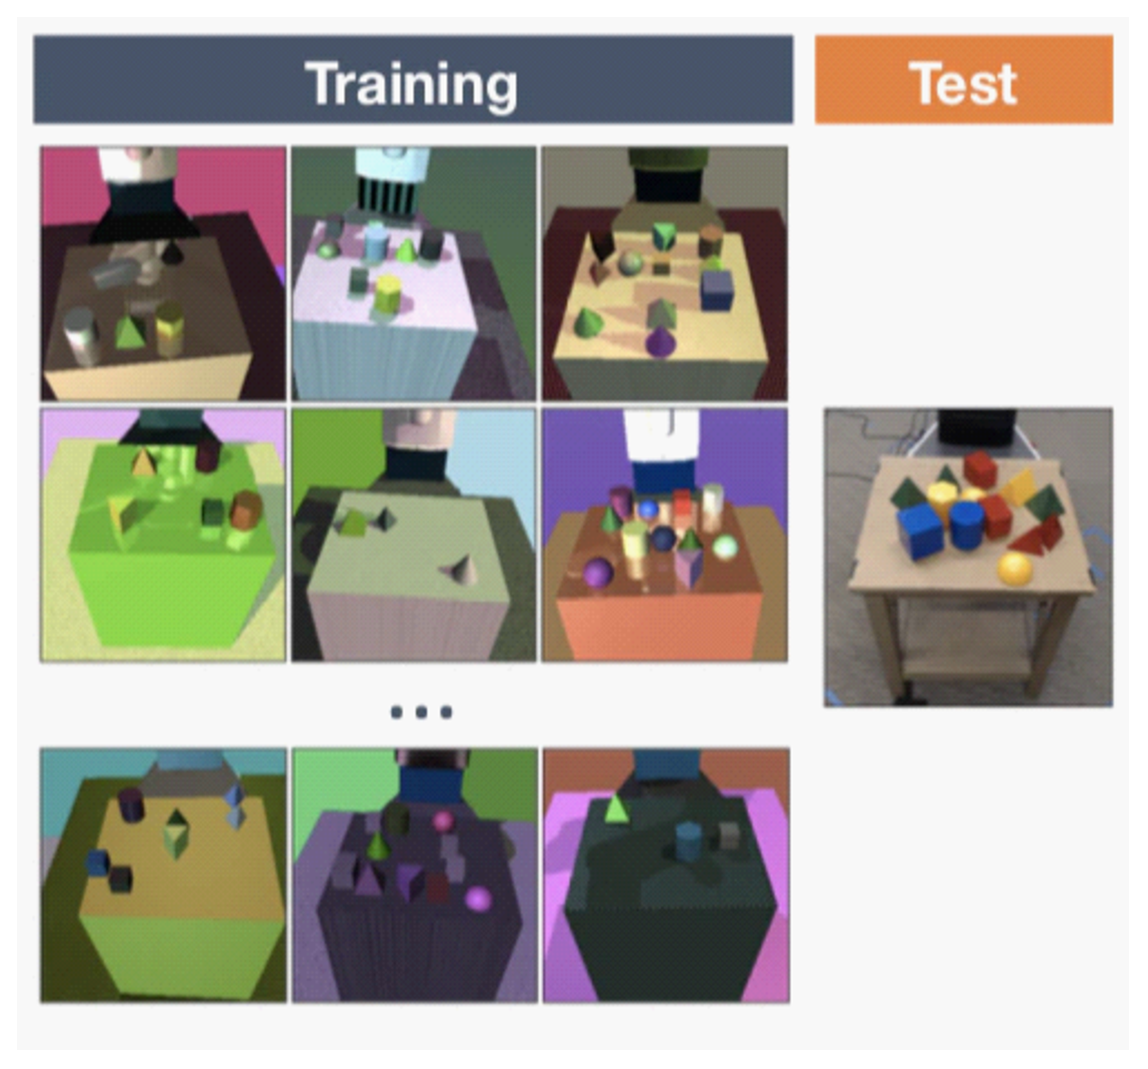
\includegraphics[width=60mm]{pic3.eps}
      \vspace*{30mm}
      \caption{Domain Randomization.}
      \label{fig:2d_pose_estimation}
      \end{figure}







\subsubsection{Autencoder}

\  今回学習に使われる手法の基礎となるのがAutencoder図4である,簡単な説明はオートエンコーダーとは、教師なし学習の一つであり,学習時の入力データは訓練データのみで教師データは利用しない,データを表現する特徴を獲得するためのニューラルネットワークである.Autencoderを表す数式を式1に示す.要素はそれぞれ x: 入力(インプット) x’:アウトプット $\phi$: エンコーダー $\psi$: デコーダー  z:潜在変数  この式のロス関数は式2に示す.



\begin{eqnarray}
\label{eq:polynomial1}
( x ^ {\prime})  = (\psi *  \phi )( x ) = \psi (z)
\end{eqnarray}


\begin{eqnarray}
\label{eq:polynomial1}
l_2=  \sum_{i \in D}\parallel{ x - x'} \parallel_2
\end{eqnarray}


     \begin{figure}[htpp]
     \centering
      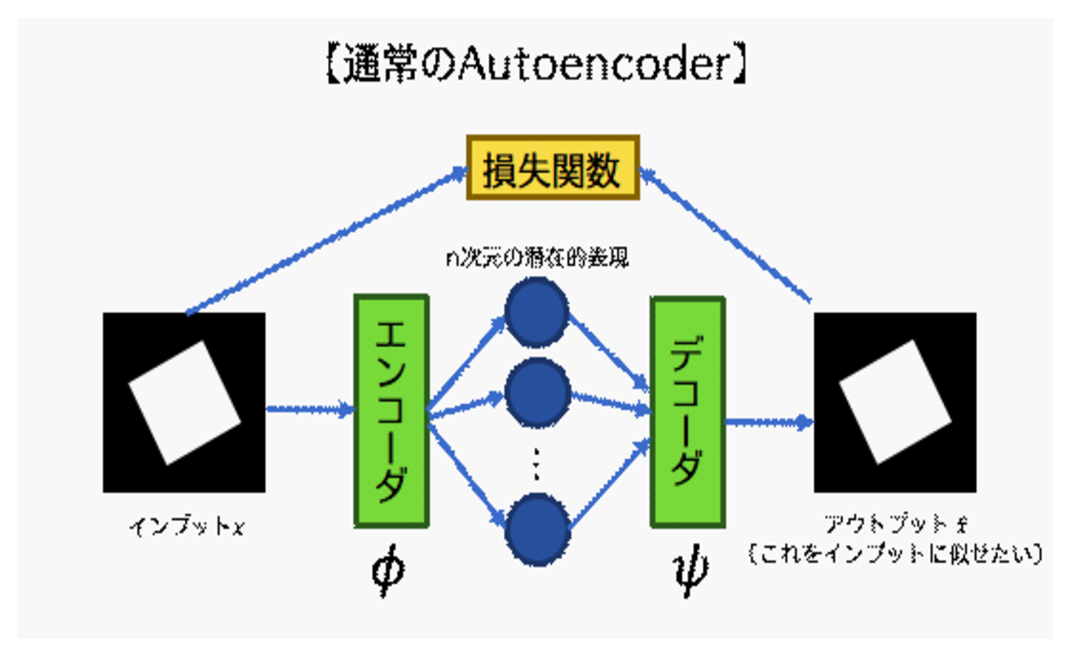
\includegraphics[width=60mm]{pic7.eps}
      \vspace*{30mm}
      \caption{Autencoder.}
      \label{fig:2d_pose_estimation}
      \end{figure}




\subsubsection{Denoising Autoencoder}
\  Autoencoderを発展させたノイズ除去方法がDenoising Autencoderである.Autoencoderにノイズありの画像を入力し、ノイズなしの画像が出力できるように学習させることで,ノイズによらない本質的な潜在表現を得ることができる方法である.


\subsubsection{Augumented Autoencoder}
\ 今回姿勢推定を行う手法で,Denoising Autoencoder,Domain Randomizationの手法を取り入れ応用したAutencoder.ノイズだけではなく背景や光、遮蔽物などの環境ノイズを追加した画像を入力し,環境ノイズなしの画像を出力できるように学習させる手法.図5\\
\ Augumented Autencoderを表す数式は,式3である.要素はそれぞれx: 入力(インプット) x’:アウトプット 𝑓𝑎𝑢𝑔𝑚 :変換(加工)の関数 x’:インプット画像を変換(加工)したもの $\phi$ : エンコーダー $\psi$: デコーダー  z:潜在変数  この式のロス関数は式2と同じである.

\begin{eqnarray}
\label{eq:polynomial1}
x ' = (\psi *  \phi * f_{augm} )( x ) = (\psi * \phi) (x'') = \psi (z)
\end{eqnarray}

    \begin{figure}[htpp]
     \centering
      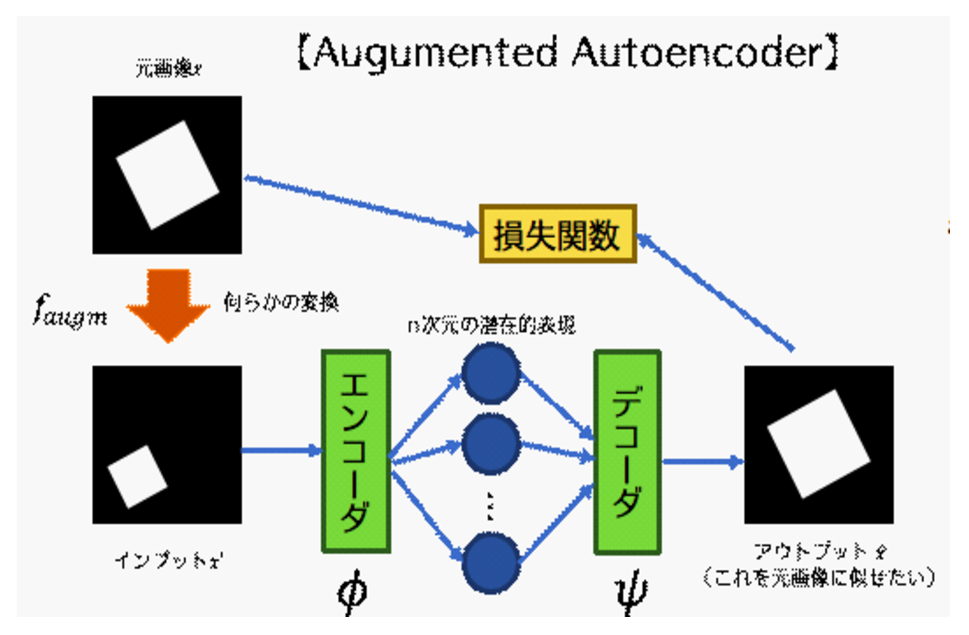
\includegraphics[width=60mm]{pic4.eps}
      \vspace*{30mm}
      \caption{Augumented Autoencoder.}
      \label{fig:2d_pose_estimation}
      \end{figure}


\subsubsection{AEとAAEの比較}
\  四角形の画像を用いた,通常のAutencoderとAugumented Autencoderの精度の比較を図5に表す.(a)をベース画像として1 : (a)→(a)   2: (d)→(d)  3: (d)→(a) の入出力で学習.結果として通常のAutencoderを使用している1・2にはあまり応用が利かず若干のノイズが入ると潜在表現を反映できないが(3)のAAEを用いたものは高精度に潜在表現を表すことができている.

    \begin{figure}[htpp]
     \centering
      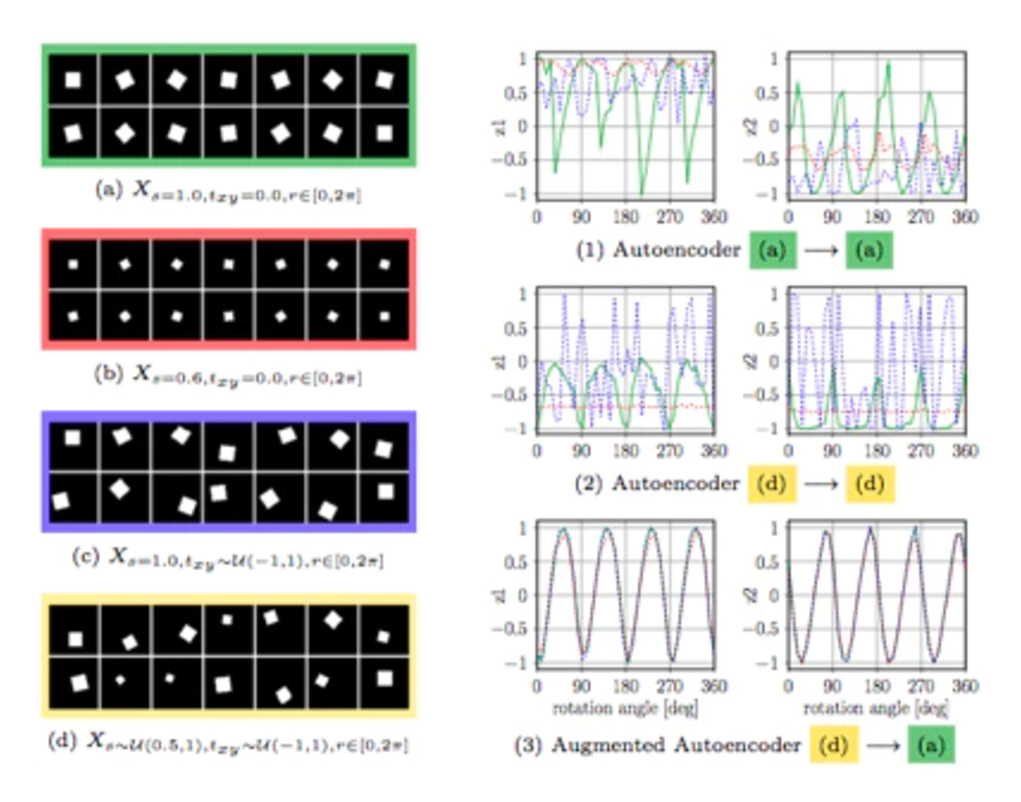
\includegraphics[width=60mm]{pic5.eps}
      \vspace*{30mm}
      \caption{,AEとAAEの比較.}
      \label{fig:2d_pose_estimation}
      \end{figure}


  


\subsection{テスト}
\  方向が既知の潜在表現と、推定したい画像から新たに得た潜在表現を比較することで,方向の推定を行う.まず,事前に学習した3Dデータから92232通りの向きの画像を作成し,それらをエンコーダに入力して学習し,潜在表現を取得する.
推定時に,SSDなどの物体検出器によって切り取られた物体画像をエンコーダに入力し潜在表現を取得,これを事前に取得した潜在表現とでコサイン類似度を測り,最も類似していたものの方向が推定したい方向となる.n次元のベクトル空間に画像を埋め込み,最近傍法を使用.92232通りというのは,球面状に均一な2562箇所の点を考え,そこに物体を36通りの回転で配置した時の球の中心からの見え方を合わせた計2562×36の92232通りである.テストの流れを図6示す.\\ 


    \begin{figure}[htpp]
     \centering
      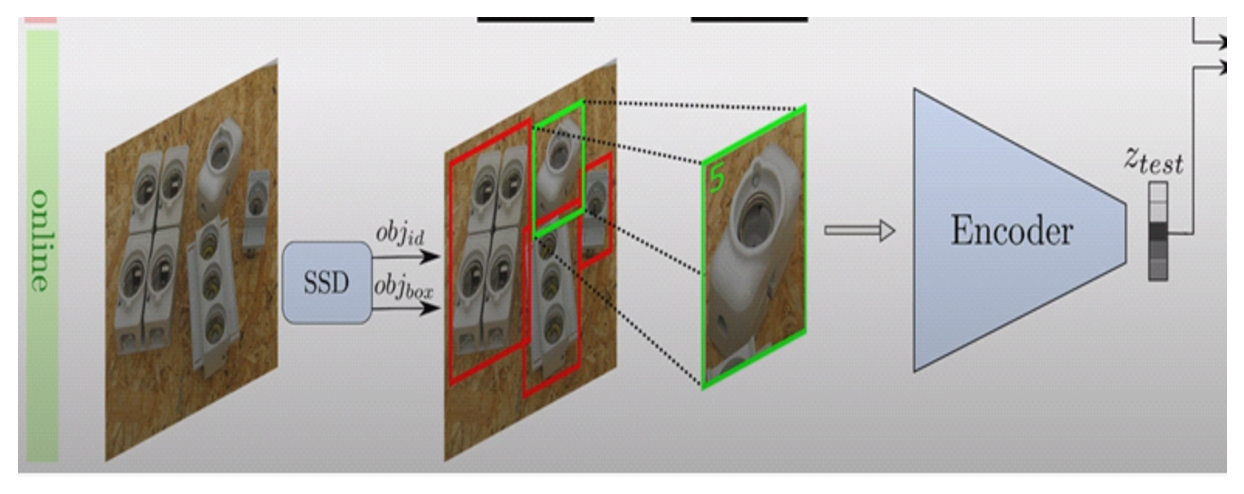
\includegraphics[width=60mm]{pic6.eps}
      \vspace*{30mm}
      \caption{テスト.}
      \label{fig:2d_pose_estimation}
      \end{figure}


\subsubsection{コサイン類似度}

\ コサイン類似度を求めるというのはトレーニングで取得し蓄積された潜在表現$ z_i $とテスト時に取得した潜在表現$z_{test}$の類似度を求める計算である.計算されたコサイン類似度の中から最も類似度の高い物(1に近い)をk近傍法によって決定する.コサイン類似度計算式は式4に示す.

\begin{eqnarray}
\label{eq:polynomial1}
cos_i = \frac {z_i * z_{test}}{|z_i||z_{test}|}
\end{eqnarray}


\subsubsection{推定}
\ 推定はコサイン類似度によって求められた最も類似度の高かった訓練データの視点,回転情報をそのままテスト時の物体の姿勢として値を返すことによって推定する.


\subsection{動作確認}


\subsubsection{動作環境}
\  \fbox{・Linux, Python 2.7  } \fbox{・Tensorflow = 1.6} \fbox{・OpenCV = 3.1}\fbox{・tensorboard ==1.6.0}\\ 
\  \fbox{・PyOpenGL==3.1.4} \fbox{・tensorflow-gpu==1.6.0} \fbox{・tensorboard ==1.6.0}\\


\subsubsection{セットアップ}

\ ・.bashrcにワークパスの設定の記述

\ \verb|AE_WORKSPACE_PATH=/path/to/autoencoder_ws|


\ ・ディレクトリの作成(ホームに作成)


\ \verb|mkdir  ae_workspace_path|

\ ・作成したディレクトリに移動しコマンドで入力

\ \verb|ae_init_workspace|

\ ・ディレクトリにファイルが生成される



\subsubsection{トレーニング}

\ ・作成されたファイルに移動し
\ ・ノイズを加えた画像の生成

\ \verb|ae_train exp_group /my_autoencoder -d|


\ ・別のターミナルでトレーニングを開始

\ \verb|ae_train exp_group / my_autoencoder|




\subsection{終わりに}
\  今調べている手法をもとに卒業研究を進めていくことに決め,方針が固まったのでゴールが明確になったという面でも先月の進捗報告会から進められていると思うので,来月までにもっとペースを上げていきたいと思っている.現在はまだ,トレーニングを行えておらずプログラムとPCと動作環境の互換性を見てGPUを使ったトレーニングを行えるようにしていかなければならない.次の進捗報告会までには,プログラムを一通り動作確認を行いそのうえでどのように自分の卒業研究につなげていけるかを考えていけるところまで進めたい.


\footnotesize

\begin{thebibliography}{9}
\bibitem{git-hub}https://github.com/DLR-RM/AugmentedAutoencoder/
\bibitem{ Implicit 3D Orientation Learning for 6D Object Detection}
https://arxiv.org/pdf/1902.01275v2.pdf/
                   



\end{thebibliography}



\normalsize

\end{document}



